% Figure D: the edit-and-continue protocol with the three interventions.
% Build: pdflatex -output-directory=/tmp fig_D.tex && cp /tmp/fig_D.pdf ../D_protocol.pdf
\documentclass[tikz,border=4pt]{standalone}
\usepackage{times}
\usepackage[T1]{fontenc}
\usetikzlibrary{positioning,arrows.meta,calc}

\definecolor{cblue}{HTML}{0072B2}
\definecolor{cverm}{HTML}{D55E00}
\definecolor{csky}{HTML}{56B4E9}
\definecolor{cgreen}{HTML}{009E73}
\definecolor{cmut}{HTML}{666666}
\definecolor{tgray}{HTML}{F0F0EE}
\definecolor{tverm}{HTML}{FBE9DE}
\definecolor{tgreen}{HTML}{E4F4EC}
\definecolor{tblue}{HTML}{E8F1F8}

\begin{document}
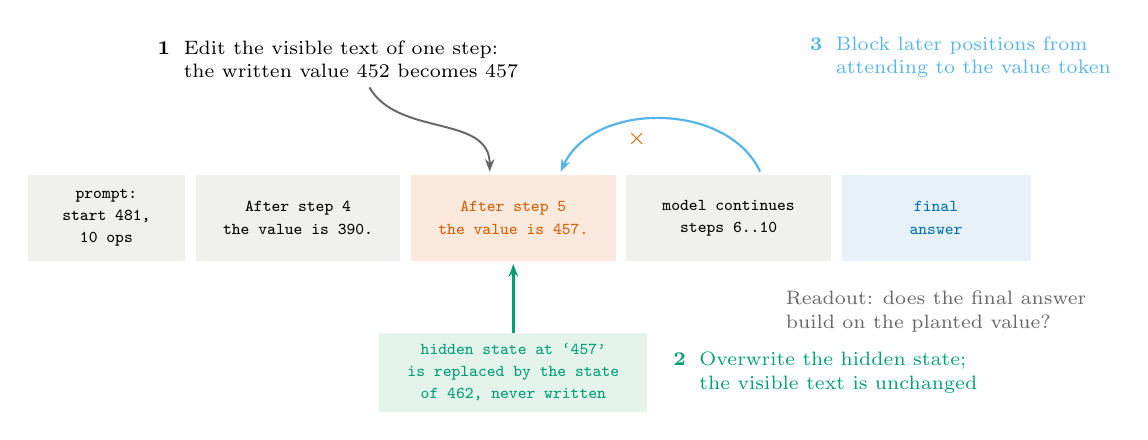
\begin{tikzpicture}[
  seg/.style={rectangle, inner sep=0pt, minimum height=11mm, align=center,
              font=\ttfamily\fontsize{6.5}{8}\selectfont, text=black},
  note/.style={align=left, font=\fontsize{7}{8.5}\selectfont},
  arr/.style={-{Stealth[length=1.6mm]}, line width=0.7pt},
  node distance=1.2mm
]

% --- the token strip: five flush segments ---
\node[seg, fill=tgray,  minimum width=20mm] (prompt)
  {prompt:\\start 481,\\10 ops};
\node[seg, fill=tgray,  minimum width=26mm, right=of prompt] (steps)
  {After step 4\\the value is 390.};
\node[seg, fill=tverm,  minimum width=26mm, right=of steps, text=cverm] (edit)
  {After step 5\\the value is 457.};
\node[seg, fill=tgray,  minimum width=26mm, right=of edit] (cont)
  {model continues\\steps 6..10};
\node[seg, fill=tblue,  minimum width=24mm, right=of cont, text=cblue] (ans)
  {final\\answer};

% --- 1: text edit (above, left) ---
\node[note, anchor=south west] (n1) at ($(steps.north west)+(-6mm,11mm)$)
  {\textbf{1}\; Edit the visible text of one step:\\
   \phantom{\textbf{1}\;} the written value 452 becomes 457};
\draw[arr, cmut] ($(n1.south)+(4mm,0)$) to[out=-60,in=90] ($(edit.north)+(-3mm,0.3mm)$);

% --- 3: attention knockout (above, right) ---
\node[note, anchor=south west, text=csky] (n3) at ($(cont.north east)+(-4mm,11mm)$)
  {\textbf{3}\; Block later positions from\\
   \phantom{\textbf{3}\;} attending to the value token};
\draw[arr, csky, line width=0.8pt]
  ($(cont.north)+(4mm,0.3mm)$) to[out=115,in=65] ($(edit.north)+(6mm,0.3mm)$);
\node[text=cverm, font=\bfseries\fontsize{8}{8}\selectfont]
  at ($(edit.north)!0.5!(cont.north)+(2mm,4.4mm)$) {$\times$};

% --- 2: state overwrite (below) ---
\node[seg, fill=tgreen, minimum width=34mm, minimum height=10mm,
      text=cgreen, below=9mm of edit] (n2box)
  {hidden state at `457'\\is replaced by the state\\of 462, never written};
\draw[arr, cgreen, line width=0.9pt] (n2box.north) -- ($(edit.south)+(0,-0.3mm)$);
\node[note, text=cgreen, anchor=west] at ($(n2box.east)+(2mm,0)$)
  {\textbf{2}\; Overwrite the hidden state;\\
   \phantom{\textbf{2}\;} the visible text is unchanged};

% --- readout ---
\node[note, text=cmut, anchor=north] at ($(ans.south)+(0,-2.5mm)$)
  {Readout: does the final answer\\build on the planted value?};

\end{tikzpicture}
\end{document}
